\documentclass[aspectratio=1610, dvipsnames, xcolor=table]{beamer}

\setbeamersize{text margin left=3mm,text margin right=3mm} 
\usepackage{t1enc}
\usepackage[magyar]{babel}
\usepackage{subcaption}
\usepackage[export]{adjustbox}
\usepackage[table]{xcolor}

\setbeamertemplate{navigation symbols}{}

\setbeamerfont{page number in head/foot}{size=\large}
\setbeamertemplate{footline}[frame number]


\definecolor{szin1}{rgb}{0.5, 0.188, 0.478}
\definecolor{szin2}{RGB}{196, 203, 133}
\definecolor{szin3}{cmyk}{0, 0.7771, 0.5437, 0.8656}
\definecolor{szin4}{gray}{0.5}

\usepackage{graphics}
\usepackage{wrapfig}

\usetheme{Pittsburgh}
\usecolortheme{crane}

\title{Féléves beadandó}
\author{Nagy Róbert és Bartók-Balogh Gábor}
\date{\today}
\subtitle{Prezentáció  \LaTeX-kel az \textbf{xcolor} csomagról}
\institute{Miskolci Egyetem}


\begin{document}
 % titleslide
    \frame[plain]{\maketitle}

        
    % slide 1 
    \begin{frame}[fragile]{Az xcolor csomag alapjai}
        \begin{minipage}{0.6\textwidth}
            \begin{itemize}
            \item \onslide<1->\verb!\usepackage[<Opciók>]{xcolor}!
            \item \onslide<2->Az xcolor lehetővé teszi, hogy kiszínezzünk szöveget,táblázatot, rajzolt ábrákat, stb... 
            \item \onslide<3->Használhatunk névvel ellátott színeket
            \item \onslide<4->Alapból 19 darab van.
            \item \onslide<5->dvipsnames opcióval 68 darab
            \item \onslide<5->svgnames opcióval 151 darab 
            \item \onslide<5->x11names opcióval pedig 317 darab
            \end{itemize}
        \end{minipage} \hfill
        \begin{minipage}{0.35\textwidth}    
            \begin{figure}
                \onslide<4->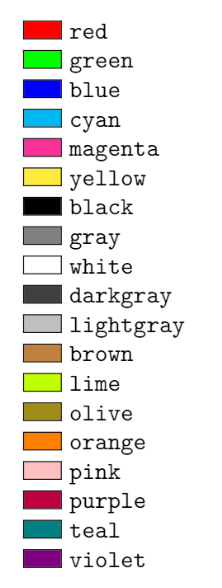
\includegraphics[scale=0.4]{img/szinek.png}
                \onslide<4->\caption{Névvel ellátott színek}
            \end{figure}
        \end{minipage}
    \end{frame}

    % slide 2
    \begin{frame}[fragile]{Saját színek}
        \begin{itemize}
            \item \onslide<1->Definiálhatunk saját színeket is.
            \item \onslide<2->\verb!\definecolor{<név>}{<Mód>}{<Értékek>}!
            \item \onslide<2->\verb!\providecolor{<név>}{<Mód>}{<Értékek>}! hasonló módon működik, de csak akkor definiálja a színt, ha az még nem létezik.
            \item \onslide<3->A mód lehet
            \begin{enumerate}
                \item \onslide<4->rgb
                \item \onslide<4->RGB
                \item \onslide<4->cmyk
                \item \onslide<4->gray    
            \end{enumerate}
        \end{itemize}                                                        
        
        \onslide<5->\begin{exampleblock}{\textcolor{white}{Példa}}
            \onslide<5->\verb!\definecolor{szin1}{rgb}{0.500, 0.188, 0.478}! \hfill \fcolorbox{black}{szin1}{ }
            \onslide<5->\verb!\definecolor{szin2}{RGB}{196, 203, 133}! \hfill \fcolorbox{black}{szin2}{ }
            \onslide<5->\verb!\definecolor{szin3}{cmyk}{0, 0.7771, 0.5437, 0.8656}! \hfill \fcolorbox{black}{szin3}{ }
            \onslide<5->\verb!\definecolor{szin4}{gray}{0.5}! \hfill \fcolorbox{black}{szin4}{ }    
        \end{exampleblock}           
    \end{frame}
    
    % slide 3
    \colorlet{mygreen}{green!40!yellow}
    \colorlet{mygreencomp}{-green!40!yellow} 

    \begin{frame}[fragile]{Színek keverése}
        \begin{itemize}
            \item \onslide<1->Keveréssel létrehozott színek mentése: \verb!\colorlet{<új szín neve>}{<keverés>}!
            \item \onslide<2->keverés kifejezés részei: $$<\text{Szín}>_1!<\text{Százalék}>_1!<\text{Szín}>_2!\ldots!<\text{Szín}>_n!<\text{Százalék}>_n$$
        \end{itemize}

        \begin{exampleblock}{\textcolor{white}{Példa}}
            \onslide<2-> \begin{verbatim}\colorlet{mygreen}{green!40!yellow}\end{verbatim} 
            \onslide<3->40\% zöld 60\% sárgával keverve \fcolorbox{black}{mygreen}{ } 
            \onslide<4->Komplementere: \fcolorbox{black}{mygreencomp}{ } \begin{verbatim}\colorlet{mygreen}{-green!40!yellow}\end{verbatim} 
        \end{exampleblock}
    \end{frame}
    
    % slide 4
    \definecolorset{rgb}{x}{10}{red,1,0,0;green,0,1,0;blue,0,0,1}

    \begin{frame}[fragile]{Színhalmazok}
        \begin{itemize}
            \item \onslide<1->Színhalmazok létrehozása: \verb!\definecolorset{<mód>}{<fej>}{<farok>}{<értékek>}!
        \end{itemize}
        \onslide<1-> \begin{exampleblock}{\textcolor{white}{Példa}}
            \verb!\definecolorset{rgb}{x}{10}{red,1,0,0;green,0,1,0;blue,0,0,1}!
        \end{exampleblock}
            
        \begin{itemize}
            \item \onslide<2-> Az így definiált színekre \textit{xred10, xgreen10} és \textit{xblue10} névvel hivatkozhatunk
            \item \onslide<3-> A \verb!\providecolorset{<mód>}{<fej>}{<farok>}{<értékek>}! hasonló módon működik, de csak akkor hozza létre a színeket, ha azok még nem léteznek.
        \end{itemize}        
    \end{frame}

    % slide 5
    \begin{frame}[fragile]{Színek tesztelése}
        \begin{itemize}
            \item \onslide<1-> A színeket a \verb!\begin{\testcolors}[<módok>]! környezetben lehet tesztelni.
            \item \onslide<1-> \verb!\testcolor{<Szín>}! használatával.
        \end{itemize}
        \onslide<1->\begin{exampleblock}{\textcolor{white}{A korábban definiált színek tesztelése Különböző módokban.}}
            \begin{verbatim}
                \begin{testcolors}[rgb,cmyk,hsb,HTML,gray]
                    \testcolor{xred10}
                    \testcolor{xgreen10}
                    \testcolor{xblue10}
                \end{testcolors}    
            \end{verbatim}    
        \end{exampleblock}
        
        \onslide<2->\begin{testcolors}[rgb,cmyk,hsb,HTML,gray]
            \testcolor{xred10}
            \testcolor{xgreen10}
            \testcolor{xblue10}
        \end{testcolors}
    \end{frame}

    %slide 6
    \begin{frame}[fragile]{Color használata}
        \begin{minipage}{0.6\textwidth}
            \begin{itemize}            
                \item \onslide<1-> színek használata: \verb!\color{<szín>}!
                \item \onslide<2-> Különböző helyeken lehet használni: szövegnél, listáknál stb...    
            \end{itemize}
        \end{minipage}
        \begin{minipage}{0.35\textwidth}
            
                \onslide<1-> például:
                \onslide<1-> \begin{verbatim}\begin{itemize}
    \color{Aquamarine}
    \item első
    \item második
\end{itemize}\end{verbatim}
                 \onslide<2-> \begin{itemize}
                    \color{Aquamarine}
                    \item első
                    \item második
                \end{itemize}
        \end{minipage}
    \end{frame}
       
    %slide 7
    \begin{frame}[fragile]{szöveg szín és háttér beállítása}
        
        \begin{itemize}            
            \item \onslide<1-> szövegszín beállítása: \verb!\textcolor{<szín>}{<szöveg>}!
            \item \onslide<1-> például: \verb!\textcolor{brown}{szöveg van itt}! = \textcolor{brown}{szöveg van itt}
            \item \onslide<2-> szövegháttér beállítása: \verb!\colorbox{<szín>}{<szöveg>}!
            \item \onslide<2-> például: \verb!\colorbox{yellow}{szöveg}! = \colorbox{yellow}{szöveg}
            \item \onslide<3-> szövegháttér + keret beállítása: \verb!\fcolorbox{<keret szine>}{<háttér szine>}{<szöveg>}!
            \item \onslide<3-> például: \verb!\fcolorbox{black}{yellow}{szöveg}! = \fcolorbox{black}{yellow}{szöveg}
            \item \onslide<4-> Az oldal háttérszínének beállítása: \verb!\pagecolor{<szín>}!
        \end{itemize}
    \end{frame}
    
    % slide 8
    \begin{frame}[fragile]{Táblázat színezés}
        \onslide<1-2>\begin{center}
            A \verb!\usepackage[table]{xcolor}! package implementálása után tudunk táblázatban is hasonló dolgokat alkotni.
            \noindent
            {\color{Dandelion} \rule{\linewidth}{1mm}}
        \end{center}
        \vfill
        \onslide<2-2>\begin{center}
            \begin{tabular}{|c|c|c|}
                \hline
                \rowcolor{Apricot}Helyezés & Versenyző & Idő \\
                \cellcolor{ForestGreen}1 & \cellcolor{Orchid}Ákos & \cellcolor{Aquamarine}1:11:210 \\
                \cellcolor{Yellow}2  & \cellcolor{Mulberry}András & \cellcolor{Emerald}1:22:156  \\
                \cellcolor{BurntOrange}3 & \cellcolor{Plum}Tomi  &  \cellcolor{PineGreen}1:30:155 \\
                \hline
            \end{tabular}
        \end{center}
    \end{frame}

    % slide 9
    \begin{frame}[fragile]{Táblázat színezés}
        \onslide<1->\begin{block}{Instukció}
            A \verb!\usepackage[table]{xcolor}! implementálás után a documentclassban meg kell adnunk a következő sort:\textbf{"xcolor=table"}
        \end{block} 
        \onslide<2->\begin{exampleblock}{\textcolor{white}{Példa}}
        {
            \verb!\documentclass[dvipsnames,xcolor=table]{beamer}!

            \verb!\usepackage[table]{xcolor}!
        }
        \end{exampleblock}	
        \begin{figure}[H]
            \onslide<2->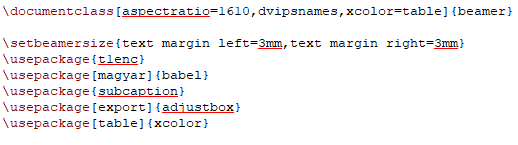
\includegraphics[scale=0.8]{img/tablesetup.png}
            \onslide<2->\caption{Felállítás}
        \end{figure}
    \end{frame}

    % slide 10
    \begin{frame}[fragile]{Táblázat színezés}
    \begin{center}
        \LaTeX-ben való alkalmazás
        \noindent
        {\color{Dandelion} \rule{\linewidth}{1mm}}
    \end{center}
    
        \begin{figure}[H]
           \onslide<2->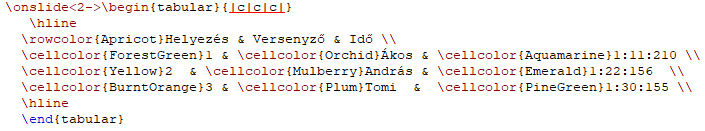
\includegraphics[scale=0.8]{img/tablealkalmazas.png}        
        \end{figure}
    \end{frame}

    
    % slide 11
    \begin{frame}[fragile]{Színsorozatok Definiálása}
        \definecolorseries{foo}{rgb}{last}{orange}{green}
        \resetcolorseries[8]{foo}
        \begin{itemize}
            \item Színsorozatok definiálása: 
            \item \begin{verbatim}\definecolorseries{<név>}{<sorozat módja>}{<metódus>}
                    [<b-mód>]{<b-szín>}[s-mód]{s-szín}\end{verbatim}
            \item A b-mód és b-szín a kezdő színt definiálják.
            \item például: [rgb]\{1,0.5,0.5\}
            \item Az s-mód és s-szín pedig meghatározza, hogy a lépésvektor hogyan lesz kiszámítva.
            \item A metódus lehet: step, grad vagy last.
        \end{itemize}
    \end{frame}

    \begin{frame}[fragile]
        \begin{itemize}
            \item \verb!\resetcolorseries[<Osztó>]{<Sorozat neve>}! Legalább egyszer használni kell. Visszaállítja a szín sorozatot és kiszámolja a lépésvektort. Az osztó egy nemnulla valós szám.
            \item step és grad esetén \{s-szín\} meghatározza a \textit{grad} irányvektort
            \item last esetén [s-mód]\{s-szín\} meghatározza a \textit{last} szín paramétervektort. (\textit{base} pedig a kezdő szín paramétervektort)    
        \end{itemize}
        \begin{center}
            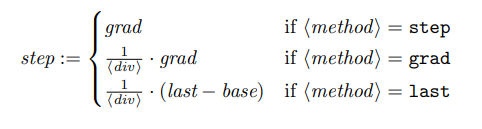
\includegraphics[scale=0.8]{img/lepesvektor.png}
        \end{center}
    \end{frame}

    \begin{frame}[fragile]{Színsorozatok használata}
        
        \definecolorseries{s1}{rgb}{step}[rgb]{.95,.85,.55}{.17,.47,.37}
        \resetcolorseries[8]{s1}
        \definecolorseries{s2}{rgb}{grad}[rgb]{.95,.85,.55}{3,11,17}
        \resetcolorseries[8]{s2}
        \definecolorseries{s3}{rgb}{last}{orange}{green}
        \resetcolorseries[8]{s3}
            \begin{itemize}
                \item \onslide<1-> \verb!\definecolorseries{s1}{rgb}{step}[rgb]{.95,.85,.55}{.17,.47,.37}!
                \item \onslide<1-> \verb!\resetcolorseries[8]{s1}!
                \item \onslide<2-> \verb!\definecolorseries{s2}{rgb}{grad}[rgb]{.95,.85,.55}{3,11,17}!
                \item \onslide<2-> \verb!\resetcolorseries[8]{s2}!
                \item \onslide<3-> \verb!\definecolorseries{s3}{rgb}{last}{orange}{green}!
                \item \onslide<3-> \verb!\resetcolorseries[8]{s3}!
                \item Sorozatok léptetése: <Sorozat név>!!+
            \end{itemize}            
    \end{frame}

    \begin{frame}{Színsorozatok példa}
        
        \begin{figure}
            \begin{center}
                \begin{subfigure}[c]{0.3\textwidth}
                
                    \rowcolors{1}{s1!!+}{s1!!+}
                    \begin{tabular}{p{2cm}}
                        \\ \\ \\ \\ \\ \\ \\ \\            
                    \end{tabular}        
                    \caption*{s1}
                \end{subfigure}
                \begin{subfigure}[c]{0.30\textwidth}
                    
                    \rowcolors{1}{s2!!+}{s2!!+}
                    \begin{tabular}{p{2cm}}
                        \\ \\ \\ \\ \\ \\ \\ \\            
                    \end{tabular}        
                    \caption*{s2}
                \end{subfigure}
                \begin{subfigure}[c]{0.3\textwidth}
                    
                    \rowcolors{1}{s3!!+}{s3!!+}
                    \begin{tabular}{p{2cm}}
                        \\ \\ \\ \\ \\ \\ \\ \\            
                    \end{tabular}    
                    \caption*{s3}
                \end{subfigure}
            \end{center}
            
            
        \end{figure}
        
    \end{frame}

    % slide 12
    \begin{frame}{Vége}
        \centering \Huge Köszönjük a figyelmet!
    \end{frame}
\end{document}